\documentclass[a4paper, 12pt]{article}
\usepackage[top=3cm, bottom=2cm, left=2cm, right=3cm]{geometry}
\usepackage[utf8]{inputenc}
\usepackage{amsmath, amsfonts, amssymb}
\usepackage{graphicx, xcolor}
\usepackage{tikz}
\usepackage{subfig}
\usetikzlibrary{arrows.meta}
\usetikzlibrary{calc}
\usepackage{scalerel, pict2e, tkz-euclide}
\usetikzlibrary{calc, patterns, arrows.meta,shadows,external}

\usepackage{pgfplots}
\usepackage{cancel}
\usepackage{enumitem}
\pgfplotsset{compat=newest}
\usepgfplotslibrary{statistics,fillbetween}
\usepackage{indentfirst}
\usepackage{babel}[pt-br]

\begin{document}

\section{Questão 1 Lista 2}

	\begin{figure}[ht]
		\centering
		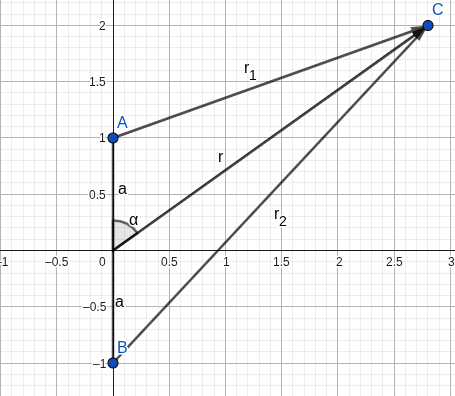
\includegraphics[width=0.5\linewidth]{Captura de tela de 2026-04-28 20-20-07.png}
	\end{figure}
	
	O potencial para um ponto $\vec{r}$ qualquer no plano será a soma das contribuições individuais de potencial de cada carga. Então:
	
	\[
	V(\vec{r})=\frac{kq}{r_1}-\frac{kq}{r_2}\]
	
	\[
	V(\vec{r})=kq\left(\frac{1}{r_1}-\frac{1}{r_2}\right)\] 
	
	\[
	V(\vec{r})=kq\left(\frac{r_2-r_1}{r_1r_2}\right)\]
	
	Para pontos distantes os vetores $\vec{r_1}$,$\vec{r_2}$ serão aproximadamente paralelos a $\vec{r}$, então a diferença entre $\vec{r_1}$ e $\vec{r_2}$ será:
	
	\begin{figure}[ht]
		\centering
		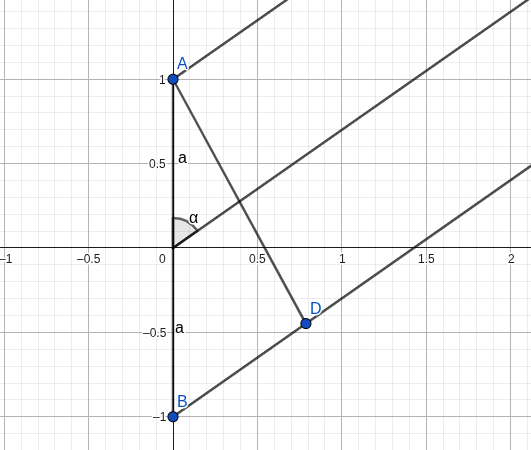
\includegraphics[width=0.5\linewidth]{figura2.png}
	\end{figure}
	
	\[
	\cos\alpha\approx\frac{r_2-r_1}{2a} \Rightarrow r_2-r_1\approx 2a\cos\alpha\]
	
	e $r_1r_2\approx r^2$, logo:
	
	\[
	V(\vec{r})\approx kq\left(\frac{2a\cos\alpha}{r^2}\right),\] $\rho=2aq\Rightarrow$ \[V(\vec{r})\approx \frac{k\rho\cos\alpha}{r^2}\] quando $r>>a$.

\section{Questão 2 Lista 2}

Como o potencial elétrico de um dipolo para grandes distâncias é dado por:
\[
V(\vec{r})\approx \frac{k\rho\cos\theta}{r^2}\]
\[
V(\vec{r})\approx \frac{k\rho y}{(x^2+y^2)^{3/2}}\]

Com isso termos o vetor campo elétrico através da relação:

\[\vec{E}=-\vec{\nabla}V\]
\[\vec{E}=\left(-\dfrac{\partial V}{\partial x}, -\dfrac{\partial V}{\partial y}\right)\] então

\[\vec{E_x}=-\dfrac{\partial V}{\partial x}\]
\[\vec{E_x}=-k\rho y\left[\frac{d}{dx}\left(\dfrac{1}{(x^2+y^2)^{3/2}}\right)\right]\]
\[\vec{E_x}=-k\rho y\left[\frac{-3}{2}\left(x^2+y^2\right)^{-5/2}2x\right]\]

\[\vec{E_x}=\frac{3k\rho xy}{(x^2+y^2)^{5/2}}\]
\[\vec{E_x}=\frac{1}{4\pi\epsilon_0}\frac{3\rho xy}{(x^2+y^2)^{5/2}}\]

\[\vec{E_y}=-\frac{\partial V}{\partial y}\]
\[\vec{E_y}=-k\rho\left[\frac{d}{dy}\left(\frac{y}{(x^2+y^2)^{3/2}}\right)\right]\]

\[\vec{E_y}=-k\rho\left[(x^2+y^2)^{-3/2}+y\frac{-3}{2}(x^2+y^2)^{-5/2}2y\right]\]

\[\vec{E_y}-k\rho\left[\dfrac{(x^2+y^2)}{(x^2+y^2)}\dfrac{1}{(x^2+y^2)^{3/2}}-\frac{3y^2}{(x^2+y^2)^{5/2}}\right]\]

\[\vec{E_y}=-k\rho\left[\frac{x^2+y^2-3y^2}{(x^2+y^2)^{5/2}}\right]\]

\[\vec{E_y}=\frac{\rho}{4\pi\epsilon_0}\left[\dfrac{2y^2-x^2}{(x^2+y^2)^{5/2}}\right]\]

\section{Questão 3 Lista 2}

A diferença de potencial entre dois pontos é:

\[V(a)-V(b)=-\int_{b}^{a}E(r)dr\]nesse caso\[V(b)-V(b+d)=-\int_{b+d}^{b}Edr\]

Calculando campo elétrico:

lei de gauss:

\[
\oint_S \vec{E}d\vec{s}=\frac{q}{\epsilon_0}\]

Como a densidade de carga é constante a carga $q$ será $q=\rho V=\rho l\pi b^2$

O fluxo será:

\[\oint_S\vec{E}d\vec{s}=2\int_{tampa}Eds\cos\theta+\int_{lateral}Eds\cos\theta\]
\[\oint_S\vec{E}d\vec{s}=El2\pi r\]$\Rightarrow$
\[El2\pi r=\frac{\rho l\pi b^2}{\epsilon_0}\]
\[E=\frac{\rho b^2}{2r\epsilon_0}\]

Utilizando em:

\[V(b)-V(b+d)=-\int_{b+d}^{b}\frac{\rho b^2}{2r\epsilon_0}dr\]

\[V(b)-V(b+d)=-\frac{\rho b^2}{2\epsilon_0}\int_{b+d}^{b}\frac{1}{r}dr\]

\[V(b)-V(b+d)=\frac{\rho b^2}{2\epsilon_0}\ln\left(\dfrac{b+d}{b}\right)\]

\section{Questão 5 Lista 2}



\section{Questão 10 Lista 2}


	\[
	P(D)=\frac{kq}{r_1}-\frac{kq}{r_2}+\frac{kq}{r_3}\]
	\[
	P(D)=\frac{kq}{r-a}-\frac{kq}{r+a}+\frac{kq}{r}\]
	
	
	\[
	P(D)=\frac{(r+a)rkq-kq(r-a)r+kq(r^2-a^2)}{(r^2-a^2)r}\]
	
	\[
	P(D)=\frac{kq\left[(r+a)r-(r-a)r+r^2-a^2\right]}{(r^2-a^2)r}\]
	
	\[
	P(D)=\frac{kq\left(r^2+ra-r^2+ra+r^2-a^2\right)}{r^3\left(1-\dfrac{a^2}{r^2}\right)}\]
	\[
	P(D)=\frac{kq\left(r^2+2ar-a^2\right)}{r^3\left(1-\dfrac{a^2}{r^2}\right)}\]
	
	\[
	P(D)=\frac{kq\left[r^2\left(1+\dfrac{2a}{r}-\dfrac{a^2}{r^2}\right)\right]}{r^3\left(1-\dfrac{a^2}{r^2}\right)}\]
	
	Se $r>>a$ então $a^2/r^2<<1$, logo:
	
	\[
	P(D)=\frac{kqr^2\left(1+\dfrac{2a}{r}\right)}{r^3}\]
	
	\[
	P(D)=\frac{kq\left(1+\dfrac{2a}{r}\right)}{r}\]
	
	\[
	P(D)=kq\left(\dfrac{1}{r}+\dfrac{2a}{r^2}\right)\]
	
	\[
	P(D)=k\left(\dfrac{q}{r}+\dfrac{2aq}{r^2}\right)\]
	
	\[
	P(D)=\dfrac{1}{4\pi\epsilon_0}\left(\dfrac{q}{r}+\dfrac{2aq}{r^2}\right)\]
	

\end{document}